\chapter{Introduction}
\thispagestyle{fancy} % this is magic. put it after every \chapter{...}
\section{Self Driving Cars}

The problem of traffic theory is generally to understand human behavior on the road and to use this knowledge for optimizing infrastructure. Determining when lanes should be added, where turns and bridges should be made, what the speed limit should be are all considerations that require engineers to turn to traffic theory. However, recent developments have raised new questions in traffic theory concerning a new kind of driver: the autonomous car. 

In theory, the efficiency of a highway system could be improved by the mere presence of these self-driving cars rather than the building of new lanes and roads. Jiang et al. \cite{jiang} cite various companies' innovations including adaptive cruise control, lane change assistance, and vehicle-vehicle communication as game changers in traffic behavior.
Holland \cite{holland} found that small disturbances in traffic flow propagate down through lanes of cars causing traffic jams, a result also found by MIT \cite{mit}. A system of cooperating self-driving cars would likely be less prone to this kind of jam propagation. This is likely to be true because self driving cars can be programmed with optimal driving strategies that do not propagate disturbances backward. One aspect of these optimal strategies would be the avoidance of causing disturbances in the first place, something human drivers can do simply by changing lanes poorly.

\section{Kerner's Three Phase Traffic Theory}
Kerner \cite{kerner} proposes that all traffic is divided into one of three states. The first state is called free flow, and it describes a state of traffic in which cars are separated far enough that drivers have no need to respond to the actions of cars around them. We assume that autonomous cars will have no effect on free flow traffic since this precludes the presence of any jam for cooperative thinking to optimize. 
 
We will instead focus on the effects of autonomous cars on the efficiency of highways in states of synchronized flow and wide moving jams which are the likely to be affected by collaborative thinking. Wide moving jams and synchronized flow are both states in which cars' movements are determined by the cars surrounding them. Kerner distinguishes the two states by how their downstream fronts propagate. A wide moving jam propagates backward at a fixed velocity while the synchronized flow phase does not.

\section{Definitions}
We choose to measure the efficiency of a highway by its throughput. Throughput is defined as the number of cars that pass through a slice of a highway in a specific period of time. We will denote throughput by the letter �q� and use cars per second as its unit of measurement. Kerner refers to this measurement as flow and sometimes as volume, but also refers to the state of traffic (free flow, synchronized flow, wide moving jam) as kinds of flow. For the sake of clarity we will refer to this measurement only as throughput in this paper.

Velocity, v, is simply the speed of a car in meters per second. Density, $\rho$, is the number of cars in a given stretch of highway and can be measured in cars per meter. Dimensional analysis tempts us to believe $q = \rho * v$, a conclusion that Kerner also arrived at.

\section{Goals and Modeling}

Our ultimate goal is to model how autonomous cars would affect traffic on the highway systems in Washington state. Given real world data about a specific highway, our model will predict the throughput of that highway with different ratios of autonomous cars.

Our model will focus on three main aspects of decision making which were pointed out by Jiang et al. to be crucial differences between human drivers and self driving cars. First, we will account for car following, which quantifies drivers’ reactions to the cars ahead of them, speeding up to close a gap or slowing down to avoid a collision. We will also model lane changing, where drivers make decisions based on cars in the next lane, possibly move into that lane, and possibly cause cars to slow down for the new driver in front of them. Lastly, since self-driving cars are capable of communicating with each other, an optimal strategy may involve hive-mind thinking.

These decisions inherently involve taking information about density and using that information to change velocity. The differences between human responses and autonomous vehicle responses to this information will affect the throughput of the highway and provide a meaningful measurement of efficiency. We expect the throughput measured in vehicles per day to not change much, because roughly the same number of people will have to commute on the highway as did before (assuming rerouting is negligible); On the other hand throughput measured in vehicles per hour during rus hour will improve, because cooperating autonomous vehicles can prevent some traffic jams by keeping a roughly constant velocity.

\section{Methodology}

In order fulfill our goal of studying the effects of autonomous cars, we want to simulate a section of highway with a program. Note that since the drivers behave differently (ie. human drivers will behave differently from autonomous drivers), we need need to simulate individual cars to find any emergent patterns. First we will find reasonable models for how humans accelerate as a function of their surroundings and how autonomous cars might accelerate as a function of their surroundings on a highway. For the former we looked at various models including Gipps \cite{gipps} and Treibar \cite{treiber}. For the autonomous we experimented with different parameters to acheive the highest traffic throughput.

Once we have a simulation, we can input real-life data as the initial conditions and general parameters (ie. vehicle density, throughput, velocity of cars) while varying the percentage of autonomous cars record the throughput, which is what we ultimately seek to maximize.

\chapter{Human Driving}
\thispagestyle{fancy} % this is magic. put it after every \chapter{...}


\section{Intelligent Driver Model}

In the literature, there are a multitude of car following models with a wide range of complexity and supporting evidence. Of these, most state of the art models defined constants whose values could be modified for realism given real data. After much testing and deliberation, we decided to use the Intelligent Driver Model described by Treiber et al. \cite{treiber}.

In this model, the acceleration of a driver depends only on the gap between himself and the car ahead of him (s), his velocity (s), and velocity difference between himself and the car ahead of him ($\Delta v$). We can describe this by the function:

$a(s, v, \Delta v) = a \left[1 - \left(\frac{v}{v_0}\right)^\delta - \left( \frac{s^*(v, \Delta v)}{s} \right)^2 \right]$

$s^*(v, \Delta v) = s_0 + vT + \frac{v\Delta v}{2\sqrt{ab}} $

This is the form given by Kesting et al. \cite{kesting}, which has an acceleration that does not exceed some desired acceleration $a$. This acceleration causes the car's velocity to approach the speed limit $v_0$ using the ratio $ 1 - \left( \frac {v} {v_0} \right) ^ \delta $ but maintains a safe distance from the car in front using the ratio $ \left( \frac {s^*( v, \Delta v )} {s} \right) ^2 $. The function $s^*$ describes the gap which the driver would find reasonable based on a minimum distance $s_0$ that a driver is willing to tolerate, a reaction time or desired time gap $T$ between the two cars, and the greatest deceleration $b$ that the driver would be willing  to tolerate comfortably. The last constant, $\delta$ describes how a driver would accelerate less at higher velocities.

Kesting et al. give values for each of these constants which they claim are reasonable, realistic, and empirically measurable:


%~ \centering
\begin{center}
\begin{tabular}{ c c c }
\hline
Parameter & Car & Unit                  \\ \hline
$v_0$     & 120 & km/h                  \\
$\delta$   & 4   &                       \\
$T$        & 1.5 & s                     \\
$s_0$     & 2.0 & m                     \\
$a$        & 1.4 & $m/s^2$ \\
$b$        & 2.0 & $m/s^2$
\end{tabular}
\end{center}

\section{Lane Changing Model}

\begin{figure}
  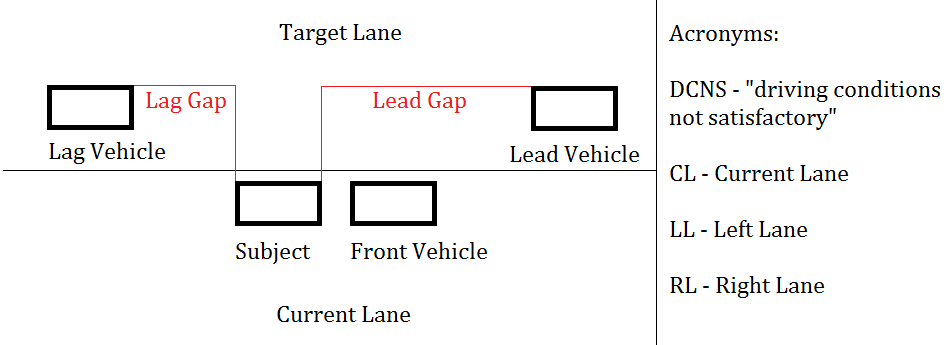
\includegraphics[width=\linewidth]{Lane_Changing_Graphic.png}
  \caption{A diagram showing several parameters for the lane-changing model.}
  \label{fig:Lane Changing}
\end{figure}

The phenomenon of lane changing by drivers is modeled probabilistically by Ahmed \cite{ahmed} in his thesis. We used that model. See Figure \ref{fig:Lane Changing} for a diagram that with following the discussion.



Here's a high-level description of the model (Here, $\nu_n$ is a standard normal variable for each person, to capture uncertainty) :

\begin{enumerate}

\item

A human decides whether or not the driving conditions in their lane are satisfactory (DCNS = �driving conditions not satisfactory�). This is given by a binary logit model.

$P_t(DCNS | \nu_n) = (1 + \exp(-X_n^{DCNS}(t)\beta^{DCNS} - \alpha^{DCNS}\nu_n)) ^ {-1}$

This is the probability that the driver finds the conditions in the current lane to be not satisfactory. That's when the driver considers a lane change. 


\item

After that, the driver looks for an acceptable gap in the neighbouring lane(s). A gap is called acceptable if the lead gap is acceptable and the lag gap is acceptable. 

The lead and lag gaps are acceptable if they each exceed the �critical' gap.

The critical gap is given by this expression:

$G_n^{cr, g} = \exp(X_n^g(t)\beta^g + \alpha^g\nu_n^g(t) + \epsilon_n^g(t)), \ g \in \{lead,\ lag\}$

Assuming $\epsilon^g_n(t) \sim N(0, \sigma_{\epsilon^g}^2)$, $G^{cr}$s are then log-normally distributed.

$P_t(gap\ acceptable) = P_t(lead\ gap\ acceptable) P_t(lag\ gap\ acceptable)$

 	$ = P(G^{lead}_n(t) > G^{cr, lead}_n(t) | \nu_n) P(G^{lag}_n(t) > G^{cr, lag}_n(t) | \nu_n) $\\
$ = P(ln(G^{lead}_n(t)) > ln(G^{cr, lead}_n(t)) | \nu_n) P(ln(G^{lag}_n(t)) > ln(G^{cr, lag}_n(t)) | \nu_n) $

$  = \Phi\left(
   \frac{
       \ln(G^{lead}_n(t)) - X_n^{lead}(t)\beta^{lead} - \alpha^{lead}\nu_n
   }{
       \sigma_{\epsilon^{lead}}
   }
\right)
\Phi\left(
   \frac{
       \ln(G^{lag}_n(t)) - X_n^{lag}(t)\beta^{lag} - \alpha^{lag}\nu_n
   }{
       \sigma_{\epsilon^{lag}}
   }
\right)
         $

\item
So then, given DCNS and $\nu_n$, the probability of switching to the left lane is given by:

         $ P_t(Left Lane (LL) | DCNS, \nu_n) = 1/(1 + \exp(-X_n^{LL}\beta^{LL} - \alpha^{LL}\nu_n)) $

\item
To put it all together:	

            $ P_t(LL | \nu_n) = P_t(gap\ acceptable for\ LL) P(LL | DCNS,\ \nu_n) P(DCNS | \nu_n) $

        $P_t(RL | \nu_n)$ can be similarly calculated, and simply, $P(CL | \nu_n) = 1 - (P_t(RL | \nu_n) + P_t(LL | \nu_n))$

\end{enumerate}

The model parameters, including which variables were the most important, and what weights/parameters to use for them, were estimated using data from Interstate 93 in Boston\cite[91]{ahmed}. Here is what we have \cite[125, 127]{ahmed}:

\noindent 

$X_n^{DCNS} =
\begin{bmatrix}
    1 \\
    \textrm{subject\ speed}\ - \textrm{desired\ speed}  \\
    \textrm{tailgate} \\ 
\end{bmatrix}
\beta^{DCNS} = \begin{bmatrix}
    0.225\\
    -0.0658\\
    0.423\\
\end{bmatrix}
\alpha^{DCNS} = -1.11\\
$

$
\noindent X_n^{lag} = \begin{bmatrix}
    1 \\
    \textrm{min(0, lag\ vehicle\ speed - subject\ speed)} \\
    \textrm{max(0, lag\ vehicle\ speed - subject\ speed)}  \\
\end{bmatrix}
\beta^{lag} = \begin{bmatrix}
    2.02\\
    0.153\\
    0.188\\
\end{bmatrix}
\begin{bmatrix}
    \alpha^{lag} \\
    \ln(\sigma_{\epsilon^{lag}})\\
\end{bmatrix} = \begin{bmatrix}
    -0.653 \\
    -0.642 \\
\end{bmatrix}\\
$

$\noindent X_n^{lead} = \begin{bmatrix}
    1 \\
    \textrm{min(0, lead\ vehicle\ speed - subject\ speed)}  \\ 
\end{bmatrix}
\beta^{lag} = \begin{bmatrix}
    0.508\\
     -0.420\\
\end{bmatrix}
\begin{bmatrix}
    \alpha^{lead} \\
    \ln(\sigma_{\epsilon^{lead}})\\
\end{bmatrix} = \begin{bmatrix}
    0.727 \\
    -0.717 \\
\end{bmatrix}
$

$\noindent X_n^{LL} = \begin{bmatrix}
    1 \\ \\
    \textrm{Lead\ vehicle\ speed - desired\ speed}  \\
    \textrm{Front\ vehicle\ speed - desired\ speed}  \\ 
    \textrm{Lag\ vehicle\ speed - subject\ speed}  \\ 
\end{bmatrix}
$
$
\beta^{LL} = \begin{bmatrix}
    -1.87\\
    0.0328\\
    -0.158\\
    -0.0960\\
\end{bmatrix}
    \alpha^{LL} = -0.246 
$

\chapter{Self Driving Car Strategies}
\section{Majority Human Traffic}

	On the topic of car following, a strategy pointed out by Grey \cite{grey} appears to be optimal for human and non-human drivers alike. The simple principle of the strategy is that drivers should stay in the midpoint of the two cars surrounding them. This gives the most room on average for drivers to brake if the car ahead of them brakes. 
The edge cases of this strategy are straightforward. A driver with no car ahead of them should only consider achieving the speed limit. A driver with no car behind need only maintain a sufficient gap to stop, similar to the human strategy's $s^*$ function.
Beaty \cite{beaty} claims that a lane change should only be made when necessary, and at the last minute. Part of his car following strategy involves the driver leaving enough room ahead of them for another car to safely change lanes into. This would prevent the backward propagation of a brake wave, or a wide moving jam as Kerner called it, because there would be no braking when a merge occurs.
The even spacing strategy would be optimal for self driving cars when the majority of drivers are human. Beaty's strategy would not be possible in an environment that includes mostly humans because humans, Beaty claims, follow a selfish strategy that tries to "punish" other drivers if they try to merge into their lane ahead of them. This claim is interestingly substantiated in the Intelligent Driver Model mentioned in the previous chapter.

\section{Hive Mind Strategies}

	The strategies above would be optimal solutions to human driving, but the human tendency to want to prevent drivers from merging ahead prevents these strategies from being implemented. Strategies that are autopilot-exclusive involve the communication between cars.
	Consider a series of self-driving cars one after the other in a single lane with no human driver between them. We will call this a platoon. Platoons can move with perfect coordination, having equal gaps between them and each gap long enough for a car to merge in.
	In traffic that contains enough self-driving cars, it is clear that these vehicles would want to form platoons by circumnavigating the human drivers around them so that they can move quickly, unhindered by human influence, but also increase safety by separating themselves from the human drivers whose ability to predict the movements of self-driving cars are hindered by the fact that their own car is not part of the hive mind.
	Platoons have several properties that can prevent traffic jams. Their even spacing allows them to prevent brake waves from forming for a short amount of time by having the front car stop at the last possible moment and each car after do the same. Since the platoon has near-instantaneous communication, this strategy affords none of the risk that would be incurred upon human drivers. When the cause of the sudden stop has ceased, the whole platoon can accelerate simultaneously and regain its gaps as its members drive forward so that no brake wave can form behind them.
	Since the simulation did not work in large scale, we can only postulate as to when platoon behaviour would become advantageous to all members of highway traffic. We are willing to postulate that this percentage is around 30 percent of vehicles on the highway being autonomous, but clearly further study is needed.

\chapter{Applying the Simulator}
\thispagestyle{fancy} % this is magic. put it after every \chapter{...}
\section{Preparing the data}

We wanted to model the traffic in a highly congested situation, so peak-hour data was best suited for it. However, the data set provided with the problem had not hourly but daily data. Hence, we decided to fetch some from the Washington State Department of Transportation's website. They have an annual Peak Hour Report, and we used the report of 2015 for our data \cite{peakhour}.\\

The report provides data for the top 200 busiest hours on various sites along our highways of interest (IS 5, 90, and 405 and SR 520). For each site, we have:\\

\noindent 1. The ID of the route it's on (e.g. Interstate 5)\\
2. The milepost.\\
3. Annual Average Daily Traffic (volume), which is basically the number of vehicles that passed that site in a given day, averaged over all the days in the last year. From that, we can extract a daily average value for flow, or cars per hour, by dividing AADT by 24 (called the AADT flow). \\
4. And we have K-factors for the top 200 busiest hours in 2015.\\ K- factor is the ratio of the cars/time (flow) in the nth busiest hour of 2015, to the AADT flow. For our simulation we used K30.\\ 
5. From the mileposts, we generated contiguous stretches along the routes using interpolation. For each such stretch, we know the flow, since we know the milepost it is centered around. Also, using the problem data, we know the number of lanes in most of these stretches, since they overlap with those in the problem data. Therefore, we have all the data we need to simulate the flow of traffic between these stretches.\\

\begin{figure}
  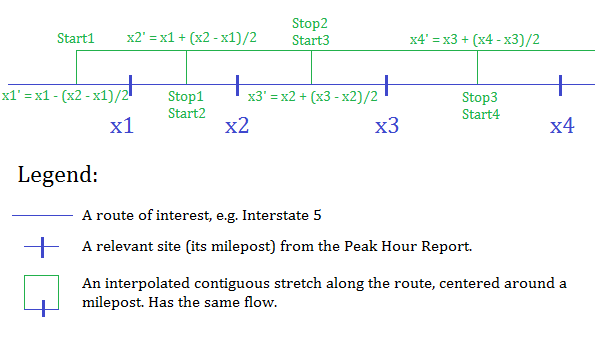
\includegraphics[width=\linewidth]{Peak_Hour_To_Stretches.png}
  \caption{How the stretches were interpolated using milepost data from the Peak Hour Report.}
  \label{fig:Peak_Hour_To_Stretches.png}
\end{figure}

We know the flow, and the number of lanes, so we can get the approximate flow per lane in each stretch. Also, this flow in one lane ($q$) must be equal to the average velocity of vehicles in that lane ($v$), times the average density of the lane ($\rho$). For simplicity, we assume that the average density and velocity of each lane is the same. $q = \rho v$\\


Here $v$ is a free variable, since we don't know how fast exactly the cars will be going. However, if we can estimate the density in a lane $\rho$, we can get an estimate for $v$. Also, we know that since peak hours are congested, $v$ is probably not close to the speed limit, and as a result, density must be quite high. First start with $\rho_{max} = 1\ car / 6\ meters$. That's a pretty packed situation, and hence we get a corresponding value for $v$, $v_{min} = q / \rho_{min}$. These are the initial conditions for our simulation. If our model of human drivers is correct, then over the course of the simulation and at the end of it, the value of the flow $q$ in the lane should be preserved. If it is not preserved, we will know that our model doesn't represent how people actually drive. (refer to Section 4.2) \\

We also know $v_{max}$, which is just the speed limit. Even though that will probably never be the average value of $v$ in a congested lane, we had anyway planned to step through the possible values of $v$ from $v_{min}$ to $v_{max}$, simultaneously stepping through $\rho_{max}$ to $\rho_{min}$, running our simulation on each $(v, \rho)$ pair. The flow $q$ should be preserved for each pair.
	 
Once we confirmed that our model of a person driving a car was accurate, we had planned to add self-driving cars to the mix. Self-driving cars follow a different strategy than the human drivers, so we expected the flow to change, because the data for the flow was generated by human drivers.

\section{Running simulations}

With a small sample (i.e. fewer cars, small road), our model preserves the flow well. But as we increase the number of cars in the simulation, the performance scales to be impractical, and we obtained unrealistic results. 

We can confidently say that the IDM model is a reasonable model for how people drive in traffic. However, we couldn't get a simulation to work well enough for us to try to mix vehicles with self-driving with it. We also couldn't get as fas as implementing lane-changing. Hence, we don't have an answer as to how self-driving cars affect the traffic on these highways.

\section{Further Research}

We need to improve our simulation so that it works to scale, and improve our model of human behaviour so that it works better when drivers are closer together. Once we can do that, we'll then implement lane-changing, and finally throw self-driving cars into the mix. After that, using the same initial conditions from the Peak Hour Report \cite{peakhour}, we can measure how the flow changes as the percentage of self-driving cars on the highway goes from 0, to 10, to 50, and to 90\%. If we observe that self-driving cars spontaneously platoon and human drivers avoid their lanes too, we can propose separate lanes for self-driving cars.

%%% Local Variables:
%%% mode: latex
%%% TeX-master: "main"
%%% End:

\begin{thebibliography}{9}

\bibitem{treiber}
	Martin Treiber, Ansgar Hennecke, and Dirk Helbing.
	Congested Traffic States in Empirical Observations and Microscopic Simulations
	Institute of Theoretical Physics, University of Stuttgart
	2000
	%~ http://journals.aps.org/pre/pdf/10.1103/PhysRevE.62.1805

\bibitem{kesting}
	Arne Kesting, Martin Treiber, and Dirk Helbing.
	Enhanced intelligent Driver Model to Access the Impact of Driving strategies on Traffic Capacity
	Institute for Transport \& Economics
	18 December 2009
	%~ https://arxiv.org/pdf/0912.3613v1.pdf

  \bibitem{gipps}
    R Eddie Wilson
    An analysis of Gipps’s car-following model of highway traffic
    Department of Engineering Mathematics, University of Bristol, Bristol BS8 1TR, UK
    IMA Journal of Applied Mathematics (2001) 66, 509–537

\bibitem{jiang}
	Tao Jiang, Srdjan Petrovic, Uma Ayyer, Anand Tolani, Sajid Husain
	Self-Driving Cars: Disruptive or Incremental?,
	Applied Innovation Review,
	Issue 1,
	June 2015.
	%http://cet.berkeley.edu/wp-content/uploads/Self-Driving-Cars.pdf

\bibitem{holland}
	E.N. Holland,
	A generalised stability criterion for motorway traffic,
	ScienceDirect,
	Volume 32,
	Issue 2
	February 1998.
	%http://cet.berkeley.edu/wp-content/uploads/Self-Driving-Cars.pdf

\bibitem{mit}
	Massachusetts Institute of Technology. 
	Mathematicians Take Aim At 'Phantom' Traffic Jams: New Model Could Help Design Better Roads.
	ScienceDaily. 
	ScienceDaily,
	14 June 2009.
	%www.sciencedaily.com/releases/2009/06/090608151550.htm

\bibitem{kerner}
	Boris S. Kerner,
	Introduction to Modern Traffic Flow Theory and Control,
	Springer,
	2009.
	%http://utdallas.primo.hosted.exlibrisgroup.com/primo_library/libweb/action/display.do;jsessionid=9F6B0DCFE6540AD9A066FCB3BF6E5A62?tabs=detailsTab&ct=display&fn=search&doc=UTD_ALMA51156292480001421&indx=1&recIds=UTD_ALMA51156292480001421&recIdxs=0&elementId=0&renderMode=poppedOut&displayMode=full&frbrVersion=&frbg=&dscnt=0&scp.scps=scope%3A%28UTD_ALMA%29&tb=t&mode=Basic&vid=UTDALMA&srt=rank&tab=catalog&vl(freeText0)=Introduction%20to%20Modern%20Traffic%20Flow%20Theory%20and%20Control&dum=true&dstmp=1484929904273

	
\bibitem{ahmed}
    Kazi Iftekhar Ahmed,
	Modeling Drivers' Acceleration and Lane-changing behavior,
	Massachusetts Institute of Technology.
	Feb 1999
	%https://its.mit.edu/sites/default/files/documents/DRIVIN.PDF%

\bibitem{peakhour}
    Washington State Dept. of Transportation,
    Peak Hour Report,
    2015
    %http://www.wsdot.wa.gov/mapsdata/travel/pdf/Peak_Hour_Report_2015.pdf%

\bibitem{kerner}
	Boris S. Kerner,
	Introduction to Modern Traffic Flow Theory and Control,
	Springer,
	2009.
	%http://utdallas.primo.hosted.exlibrisgroup.com/primo_library/libweb/action/display.do;jsessionid=9F6B0DCFE6540AD9A066FCB3BF6E5A62?tabs=detailsTab&ct=display&fn=search&doc=UTD_ALMA51156292480001421&indx=1&recIds=UTD_ALMA51156292480001421&recIdxs=0&elementId=0&renderMode=poppedOut&displayMode=full&frbrVersion=&frbg=&dscnt=0&scp.scps=scope%3A%28UTD_ALMA%29&tb=t&mode=Basic&vid=UTDALMA&srt=rank&tab=catalog&vl(freeText0)=Introduction%20to%20Modern%20Traffic%20Flow%20Theory%20and%20Control&dum=true&dstmp=1484929904273

\bibitem{grey}
	CGP Grey
The Simple Solution to Traffic
YouTube
2016

\bibitem{beaty}
William J. Beaty
Merging Lane Traffic Jams: A Simple Cure
trafficwaves.org
1998

\end{thebibliography}

%%% Local Variables:
%%% mode: latex
%%% TeX-master: "main"
%%% End:
